% Overleaf/LaTeX draft of the manuscript, converted from Manuscript_Draft.md.
% Uses the standard article class (not MDPI's proprietary class file) so it
% compiles immediately on Overleaf with zero extra setup. For final MDPI
% submission, copy each section's body text into MDPI's official Overleaf
% template (search "MDPI" in Overleaf's Template Gallery) -- the content
% below is already organized to match MDPI's Front Matter / Body / Back
% Matter structure, so that transplant should be mostly copy-paste.
%
% Deliberately NOT carried over from the markdown draft: the "pass N" / "NEEDS
% ATTENTION" / Open Items scaffolding, which documents our own editing process
% and does not belong in any version of the actual manuscript. Genuine unresolved
% items that would otherwise be silently lost are kept as %TODO comments (invisible
% in the compiled PDF) or, where leaving something blank would be worse than a
% visible placeholder, as bracketed text like [CONFIRM AFFILIATION].
%TODO: institution/affiliation, funding statement, author-contribution role
% split, and a Zenodo DOI for the code repo are still open -- see the chat
% history / Manuscript_Draft.md's Open Items for full context.

\documentclass[11pt]{article}
\usepackage[margin=2.5cm]{geometry}
\usepackage{graphicx}
\usepackage{booktabs}
\usepackage{amsmath}
\usepackage{amssymb}
\usepackage[colorlinks=true,linkcolor=blue,citecolor=blue,urlcolor=blue]{hyperref}
\usepackage{authblk}
\usepackage{caption}
\usepackage{setspace}
\onehalfspacing

\title{\textbf{Knowledge Tracing and Adaptive Difficulty for Serious Games: Design and Simulation-Based Evaluation on an Immune System Education Game}}

\author[1]{Hanan M. Helwa}
\author[1]{Osama Taha}
\author[1,*]{Adel Taweel}
\affil[1]{[Department, University, City, Country --- CONFIRM]} %TODO: affiliation
\affil[*]{Correspondence: [email --- CONFIRM]} %TODO: email

\date{}

\begin{document}
\maketitle

\begin{abstract}
\noindent
Serious games typically apply a fixed level and difficulty progression regardless of what an individual learner has understood. This paper presents a serious-game AI layer coupling per-learner Bayesian knowledge tracing over a small set of curriculum concepts with a bandit-based adaptive difficulty controller. We evaluate it using Immune Soldiers, our own prior serious game for immune-system education, whose client is only partially implemented: 200 synthetic learners with heterogeneous skill, learning, and forgetting rates played 120 encounters across its five knowledge concepts, under the game's original fixed progression, a random-difficulty ablation, and full adaptation. The original progression leaves one concept, mismatched to a permanently high difficulty, severely under-mastered; the adaptive system equalizes final mastery across all five. A well-tuned fixed difficulty, tested separately, closes most of this gap alone and matches the adaptive system's mastery and calibration; the adaptive system's remaining advantage is lower frustration and a smaller residual equity gap from personalizing to each learner, not higher achievement overall. The ablation isolates difficulty-tier adaptation, not concept selection, as that advantage's source; even so, the system still declares roughly one in six concepts mastered prematurely. Estimates correlate moderately with true mastery, indicating calibration against real classroom data is needed before deployment.
% Title and Introduction generalized to match this framing (see Section 1) -- resolved, not left open.
\end{abstract}

\noindent\textbf{Keywords:} serious games; adaptive learning; knowledge tracing; dynamic difficulty adjustment; intelligent tutoring systems; immunology education; game-based learning

\section{Graphical Abstract}
\begin{figure}[h]
\centering
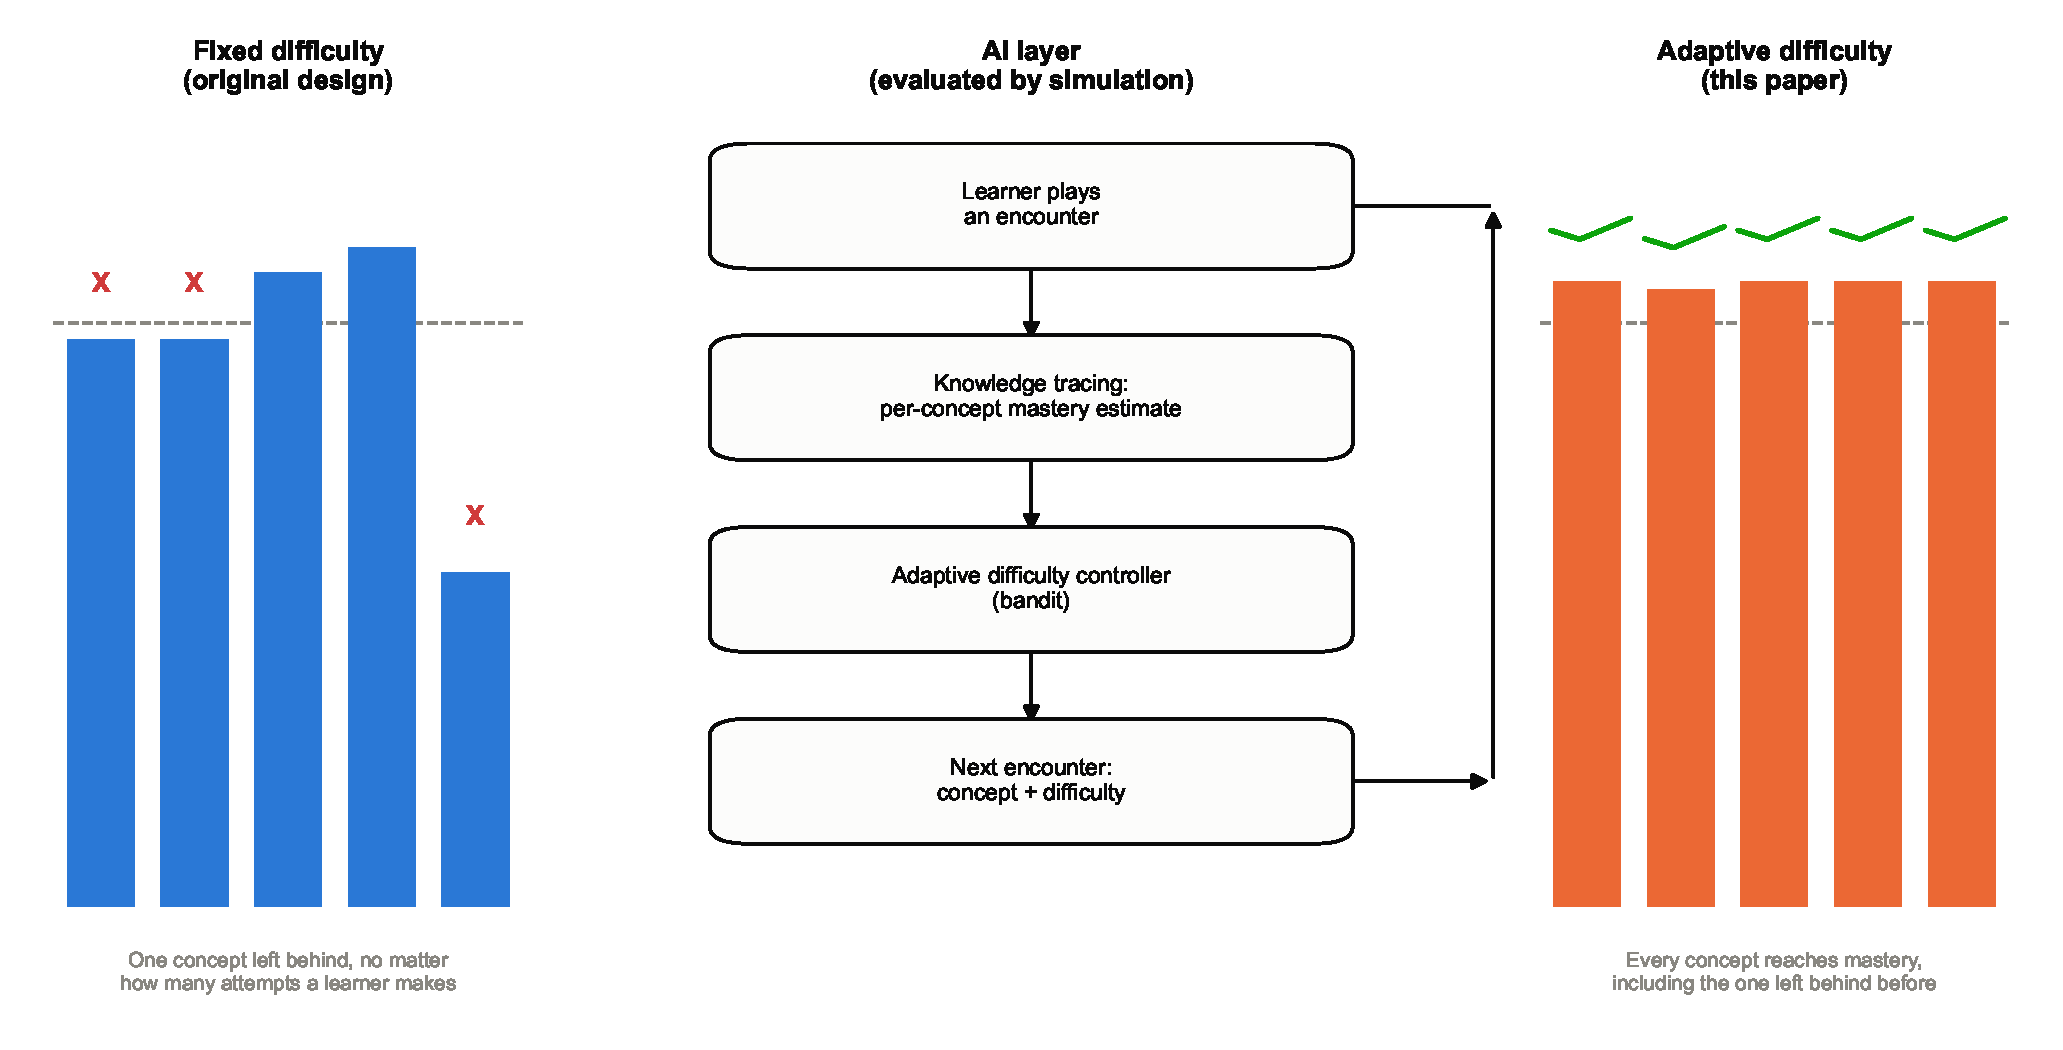
\includegraphics[width=\textwidth]{figures/graphical_abstract.pdf}
\end{figure}

\section{Introduction}

Artificial Intelligence (AI) is no longer an abstract promise for the future of education; advances in machine learning, reinforcement learning, and generative modeling are actively reshaping how learning content is created, mediated, and adapted to individual learners \cite{ref1,ref2}. Serious games and game-based learning environments occupy a distinctive position within this shift. Unlike static instructional media, games generate continuous streams of fine-grained behavioral data -- actions, choices, failures, retries -- that make them natural testbeds for adaptive and AI-driven educational systems, where algorithmic models of the learner can be coupled directly to the mechanics the learner is interacting with \cite{ref3,ref4}. Realising this potential, however, requires more than embedding a game in a curriculum: it requires computational infrastructure capable of modeling what a learner knows and translating that model into moment-to-moment changes in gameplay.

A recurring limitation across serious games generally is that ``AI'' in the game-design sense refers to scripted, non-adaptive enemy behavior -- finite-state agents that pursue or attack the player within a fixed range -- rather than AI in the AIED sense of a model that represents what the learner currently understands and adapts the experience accordingly. Content in this class of game is generally authored once and applied uniformly to every player, which the wider games-adaptivity literature has identified as a persistent source of predictable, impersonal gameplay and limited real-time instructional adaptation \cite{ref3,ref24}. Difficulty typically increases on a fixed schedule (e.g., stage 1 $\to$ stage 2 $\to$ boss) regardless of whether the individual learner has actually grasped the underlying concept that stage was designed to teach. As a result, two learners who finish the same level may leave with very different levels of conceptual mastery, and the game has no way of knowing this, let alone responding to it. This is precisely the gap the AIED literature on learner modeling, knowledge tracing, and dynamic difficulty adjustment (DDA) has targeted in other domains \cite{ref16,ref17,ref22}, but it has rarely been applied, in an explicit and evaluable form, within a real serious game's own concept and level structure.

We ground this investigation in a concrete serious game rather than a synthetic testbed, and choose immunology education as the specific domain because it is one where this gap is especially acute. Immunology is widely reported as one of the more difficult subjects for learners to build a coherent mental model of: its objects (cells, signaling molecules, receptors) are invisible and abstract, its vocabulary is dense, and it spans multiple biological scales in a way that invites memorization of disconnected facts rather than systems-level understanding \cite{ref5}. Serious games have been proposed as a way to make these processes tangible by casting immune cells and pathogens as game entities that learners control or oppose, allowing learners to experience the logic of an immune response rather than memorize it \cite{ref6,ref7}. Notable examples include \textit{Immune Attack} \cite{ref8}, developed by the Federation of American Scientists to teach cellular immunology concepts to learners across grades 5--12 through a 3D simulation in which the player guides white blood cells against invading bacteria -- consistent with the grades 5--12 evaluation population reported in Section 2.1 \cite{ref28}, rather than high-school students specifically; \textit{Cell Studio} \cite{ref6}, a client--server 3D simulation platform (built on the Unity engine) that models immunological processes at the cellular level with biophysical rules; and \textit{Cells of War} \cite{ref7}, a card-based serious game familiarizing players with immune-system functions and disease mechanisms. Our own prior work, \textit{Immune Soldiers}, follows this pattern: a Unity3D side-scrolling action game in which the player controls immune cells (macrophages, B cells, T helper and T cytotoxic cells) across levels corresponding to stages of an immune response, aimed at learners aged 8--16 \cite{ref9} -- and is the specific game this paper's AI layer is built for and evaluated on (Section 3.1).

This paper addresses the general gap identified above. We present the design and implementation of an AI layer that sits between the learner and a serious game and consists of two coupled components: (1) a \textbf{knowledge tracing model} that estimates, per learner and per curriculum concept, the probability that the concept has been mastered, using in-game evidence (quiz/dialogue responses, deaths, retries, and time-on-task) rather than a single end-of-level score; and (2) an \textbf{adaptive difficulty controller} that consumes the current mastery and engagement estimates and selects gameplay parameters -- enemy health and damage, spawn rate, hint frequency, in-game quiz difficulty -- for the encounter the learner is about to face. In this paper's instantiation, the two components are connected to five knowledge components (innate immunity, antigen recognition, cell-mediated immunity, humoral immunity, and immunological tolerance/autoimmunity) that map directly onto Immune Soldiers' own character roster and level structure, so that each in-game entity (Macrophage, B cell, T helper cell, T cytotoxic cell, Invader) doubles as a diagnostic signal for one concept.

Because deploying an untested adaptive system directly with children raises both feasibility and ethical questions that are outside the scope of a first technical contribution, we evaluate the system through simulation: synthetic learner agents, parameterized by initial skill, learning rate, and forgetting rate, are played through an abstracted version of the level/boss loop under both the adaptive controller and a fixed-schedule baseline equivalent to the original game design. This lets us report reproducible, quantitative results on mastery-convergence speed and challenge--skill balance without requiring human-subjects data collection, while positioning a classroom pilot with real learners as the natural next step.

In summary, this paper makes the following contributions:

\begin{itemize}
\item \textbf{An AI layer design for serious games}, coupling a two-channel knowledge tracing model with an adaptive difficulty controller, specified in enough architectural detail (Section 3) to be integrated into an existing Unity-based game once its client-side implementation is complete.
\item \textbf{A simulation-based evaluation methodology} that allows an AI-driven adaptation mechanism to be validated against synthetic learners with heterogeneous skill, learning, and forgetting dynamics before a full game client or real learner population is available -- a reusable pattern for AIED-in-serious-games work more generally, where a complete, deployable game is often the bottleneck to any evaluation at all.
\item \textbf{An empirical demonstration of a specific failure mode in fixed-difficulty game design, and a precise account of what adaptivity actually fixes about it.} A concept permanently assigned to a high difficulty tier is left severely under-mastered regardless of how many attempts a learner makes (Section 4.3), and mastery-based concept sequencing corrects this specific failure (Section 4.4). We then show (Section 4.8) that most of this failure was an avoidable design choice rather than an inherent property of non-adaptive difficulty: a single well-chosen fixed difficulty closes most of the same gap and even exceeds the adaptive system on mean final mastery and calibration. What the adaptive system still provides beyond a well-tuned fixed policy is narrower and more specific -- lower frustration and a smaller residual equity gap attributable to per-learner personalization -- and we report that narrower, more defensible claim rather than the broader one a comparison against only the original (mismatched) baseline would have supported.
\item \textbf{An ablation isolating the source of the adaptive system's efficiency and engagement gains} to the difficulty-tier controller specifically, showing that concept sequencing alone (without difficulty adaptation) achieves the same equity outcome far less efficiently and with substantially higher simulated frustration.
\item \textbf{A methodological caution for knowledge-tracing-driven adaptive systems}: an estimator that is only moderately calibrated against ground-truth mastery can cause a sequencing policy to withdraw instruction prematurely, and we quantify this directly -- a single-crossing mastery rule is premature 92.8\% of the time in this setting; requiring ten consecutive above-threshold observations substantially reduces but does not eliminate this (15.4\%) -- a design detail, and a residual open problem, with implications beyond this specific game.
\end{itemize}

The remainder of the paper is organized as follows. Section 2 reviews related work. Section 3 describes the system design. Section 4 reports the simulation-based evaluation. Section 5 discusses implications and limitations. Section 6 concludes.

\section{Related Work}

\subsection{Serious games for biology and immunology education}

Serious games -- defined by Abt as games with ``an explicit and carefully thought-out educational purpose'' \cite{ref13} and popularized in the education and training space by Sawyer and Rejeski \cite{ref14} and Michael and Chen \cite{ref15} -- have been widely applied to biology education, where abstract or microscopic processes benefit from a concrete, interactive representation. A 2025 systematic review of serious games across STEM education more broadly, covering 37 studies, confirms this remains an active and growing area rather than a settled one, while also noting persistent gaps in rigorous evaluation methodology across the field \cite{ref31} -- a gap this paper's simulation-based evaluation (Section 3.5) and multi-seed robustness checks (Section 4.6) are a partial response to, even if only in simulation. Narrowing to the health domain specifically, a 2025 meta-review of AI applications in health-focused serious games (2017--2025) identifies adaptation and personalization as the AI capability most frequently pursued in this space, but reports comparatively few implementations that pair that adaptation with a formal learner model of the kind knowledge tracing provides \cite{ref36} -- the specific combination this paper investigates. Within immunology specifically, \textit{Immune Attack} \cite{ref8} is the most cited example, evaluated in grades 5--12 classrooms across the United States between 2009 and 2013, with a reported comparison of 180 players against 142 students who played a control game \cite{ref28}. \textit{Cell Studio} \cite{ref6} and \textit{Cells of War} \cite{ref7} extend this space with different mechanics and fidelity trade-offs -- the former a research-oriented, biophysically grounded simulation platform, the latter a lighter card-game format -- but share with \textit{Immune Attack} and our own prior design \cite{ref9} a single-pass, authored-difficulty structure. Design frameworks for this space, such as the Learning Mechanics--Game Mechanics mapping proposed by Arnab et al. \cite{ref11} and the essential-features framework for serious games design by Lameras et al. \cite{ref12}, emphasize that the pedagogical value of a serious game depends on tight alignment between the mechanic and the concept it represents, and on formative feedback loops that let the game respond to the learner's developing understanding rather than only to task completion.

What is largely absent from this line of work, including in the design of our own prior game \cite{ref9}, is an explicit, updatable model of learner knowledge that is used to drive gameplay. Difficulty and content progression are typically authored once, at design time, and applied uniformly to every player; the ``response'' a game makes to a struggling learner is usually limited to allowing retries rather than to changing what is being asked of them. This paper treats that authoring-time design as a baseline to be compared against, not as the finished contribution.

\subsection{Learner and knowledge modeling}

Learner modeling is the AIED problem of inferring, from observed behavior, latent quantities such as a learner's mastery of specific concepts. The dominant family of approaches for concept-level mastery estimation is knowledge tracing. Bayesian Knowledge Tracing (BKT) \cite{ref16} models each skill as a binary latent state (mastered/not mastered) updated via a Hidden Markov Model from sequences of correct/incorrect responses, and has been the basis for adaptive sequencing in intelligent tutoring systems for over two decades, with meta-analytic evidence that well-built ITS approach the effectiveness of human tutors \cite{ref17}. Deep Knowledge Tracing (DKT) \cite{ref18} replaced the HMM with a recurrent neural network to model dependencies across multiple skills jointly, at the cost of interpretability and of requiring substantially more training data than a single classroom deployment typically provides -- a trade-off explicitly discussed in the knowledge-tracing survey literature, which notes that simpler probabilistic models such as BKT remain more data-efficient and more stable under limited or shifting data than deep sequence models, which need larger datasets to realize their accuracy advantage \cite{ref19}. The field has continued to move well beyond DKT since: a 2025 technical survey identifies attention-based, graph-structured, memory-augmented, and explainability-oriented knowledge tracing models as the current state of the art, with attention-based variants reported as the most stable under noisy or shifting input \cite{ref29}. Given the scale of a serious-game deployment (a handful of concepts, per-learner online updating, and a strong preference for an auditable model when the domain is a science curriculum), we adopt a BKT-style formulation per knowledge component rather than any of these more capable but more data-hungry and less transparent alternatives.

A separate and, for this paper, directly relevant strand of the knowledge-tracing literature examines \textit{equity} and \textit{fairness} in these models rather than only predictive accuracy: BKT-based mastery estimates have been shown to differ systematically across learner subgroups with equal underlying ability but different auxiliary characteristics, such as reading ability in a math-tracing context \cite{ref34,ref35}, and an ``equitable tutoring system'' has been characterized as one that reaches maximum knowledge in minimal time \textit{for every learner}, not only on average \cite{ref34}. That literature examines equity \textit{across learners} for a single skill; the equity finding at the center of this paper (Section 4.4) is, by contrast, equity \textit{across concepts} for a given learner -- a knowledge-tracing-driven system that serves five concepts unevenly, leaving one badly under-mastered while others are served well. To our knowledge this concept-level framing of equity has not been previously reported for a knowledge-tracing-driven serious game, and Section 5.1 returns to this connection once the finding itself has been presented.

Engagement and affect modeling -- inferring boredom, frustration, or flow from behavioral signals during learning \cite{ref20}, including deliberate ``gaming the system'' behavior that undermines an ITS's ability to infer true mastery \cite{ref21} -- is a closely related strand of learner modeling that several AIED systems combine with knowledge tracing to decide not just \textit{what} a learner has mastered but \textit{how} to intervene. We use a lightweight behavioral proxy for engagement (retry rate, response latency) rather than physiological or facial signals, to avoid the additional data-collection and consent burden such signals typically introduce, particularly with a target age range of 8--16.

\subsection{Dynamic difficulty adjustment and adaptive scaffolding in games}

Dynamic difficulty adjustment (DDA) -- algorithmically varying game parameters in response to player performance -- has been studied extensively in the games literature, from Hunicke's early formulation of the case for DDA and the \textit{Hamlet} system \cite{ref22} to later surveys covering rule-based, model-based, and reinforcement-learning approaches \cite{ref23,ref24}. Reinforcement learning framings typically treat difficulty selection as a sequential decision problem where the reward reflects some notion of maintained challenge or flow -- recent work continues to develop this line directly, for example continuous RL-based difficulty adjustment tailored to a player's trial-by-trial performance in a working-memory game \cite{ref30}; contextual bandit formulations are a common simplification when the action space (a small set of difficulty settings) and the feedback signal are simple enough that the full sequential-credit-assignment machinery of RL is not required \cite{ref25}. Bandit-based DDA has the practical advantage of being analyzable and tunable with far less data than deep RL, at the cost of not planning over multi-step consequences -- an acceptable trade-off for per-encounter difficulty selection of the kind used here. At the systems level, a 2024 framework for adaptive serious games similarly argues for decoupling the adaptation logic from the game client as a distinct architectural layer \cite{ref37}, the same separation this paper's architecture adopts (Section 3.4).

A small number of recent serious-game studies have coupled AI-driven adaptation directly to measured learning outcomes rather than only to raw performance -- for example, AI-generated verbal and visual scaffolding delivered by a non-player character in a physics-themed serious game, shown to affect both learning gains and cognitive load \cite{ref10}. This confirms that coupling AI adaptation to learning-relevant state (rather than score alone) is both feasible and measurable, but such systems remain rare, and none of the examples identified here drive that adaptation from a concept-level knowledge-tracing model of the kind used in intelligent tutoring systems. Within educational games specifically, DDA has mostly been applied to generic performance signals (score, completion time) rather than to concept-level mastery estimates. Coupling the two -- using \textit{what the learner has and has not learned}, rather than \textit{how well they are currently performing}, as the input to a difficulty controller -- is the combination this paper investigates, applied to the immune-system domain via the five-concept map introduced in Section 3.

\subsection{Positioning of this work}

Taken together, the literature establishes (i) serious games as an effective but typically non-adaptive medium for immunology education, (ii) knowledge tracing as a mature, interpretable approach to concept-level learner modeling, and (iii) DDA/bandit methods as a tractable way to turn a learner model into moment-to-moment gameplay changes. This paper's contribution is the integration of these three lines -- a knowledge-tracing-driven difficulty controller, mapped onto an existing immune-system game's concept and character structure, evaluated through simulation -- rather than an advance within any one of them individually.

\section{System Design and Implementation}

\subsection{Base game and knowledge-component map}

We treat \textit{Immune Soldiers} \cite{ref9} as the design source rather than a finished runtime: its scientific content, character roster, and level/boss structure define the domain and the game-facing vocabulary the AI layer operates on, while the AI layer itself is implemented and evaluated independently of the current (partially built) Unity client (Section 3.4).

The game's scientific background \cite{ref9} and character roster decompose naturally into five knowledge components (KCs), each already represented by a distinct in-game entity or encounter type (Table~\ref{tab:kcmap}).

\begin{table}[h]
\centering
\caption{Knowledge components and their in-game representation.}
\label{tab:kcmap}
\begin{tabular}{@{}lll@{}}
\toprule
KC & Concept & In-game representation \\
\midrule
KC1 & Innate immunity & Early-level Macrophage encounters \\
KC2 & Antigen recognition & Invader-identification encounters \\
KC3 & Cell-mediated immunity & T helper / T cytotoxic cell levels \\
KC4 & Humoral immunity & B cell / antibody-arrow levels \\
KC5 & Immunological tolerance \& autoimmunity & Late-game boss encounters \\
\bottomrule
\end{tabular}
\end{table}

The original design fixes the order in which these are encountered (three stages per level, a mid-level boss, a final boss) and applies one difficulty setting to every player who reaches a given stage. We generalize this into a \textbf{pool of encounters}, each tagged with a primary KC and a difficulty tier (Easy / Medium / Hard, realized as concrete Unity parameters: enemy health and damage multipliers, spawn rate, hint frequency, and in-game quiz-bank difficulty). The original fixed progression is retained unmodified as the \textbf{static baseline} condition (Section 3.5); the pool structure is what the adaptive controller (Section 3.3) selects from. This reframing -- from an authored sequence to a selectable pool -- is itself a small but necessary design change to the original game, and is called out explicitly here rather than left implicit, since Section 5 revisits it as a limitation relative to the currently implemented (Level 1 only) build.

\subsection{Knowledge tracing model}

For each KC $k$ and learner, we maintain a latent binary mastery state and track $P(L_{k,t})$, the estimated probability of mastery after the $t$-th opportunity to demonstrate KC $k$. We use a Bayesian Knowledge Tracing (BKT) formulation \cite{ref16} with the standard four parameters per KC -- prior mastery $P(L0_k)$, learning rate $P(T_k)$, guess rate $P(G_k)$, and slip rate $P(S_k)$ -- chosen over a deep sequence model (e.g., DKT \cite{ref18}) for the interpretability and data-efficiency reasons discussed in Section 2.2 \cite{ref19}.

\textbf{Evidence.} Unlike a classic ITS, an encounter yields more than one observation channel: a quiz/dialogue response (correct/incorrect) and a combat outcome (encounter cleared / player defeated). We treat these as two independent emission channels of the same latent mastery variable, each with its own guess/slip pair ($P(G_{quiz}), P(S_{quiz})$ and $P(G_{combat}), P(S_{combat})$), updated with whichever channel(s) fired during that encounter. This is a modest application of an existing idea rather than a new algorithm family: item-conditioned, multiple guess/slip parameter sets (``multi-guess, multi-slip'') are a documented BKT extension, implemented for example in the widely used pyBKT library \cite{ref32}; our two-channel setup is a direct instance of this pattern with ``channel'' (quiz vs.\ combat) taking the role item type plays in that literature.

\textbf{Update rule}, applied per channel $c \in \{quiz, combat\}$ that produced an observation at opportunity $t$:

\begin{equation}
P(L \mid \text{correct}) = \frac{P(L_{t-1})\,(1 - P(S_c))}{P(L_{t-1})\,(1 - P(S_c)) + (1 - P(L_{t-1}))\,P(G_c)}
\end{equation}
\begin{equation}
P(L \mid \text{incorrect}) = \frac{P(L_{t-1})\,P(S_c)}{P(L_{t-1})\,P(S_c) + (1 - P(L_{t-1}))\,(1 - P(G_c))}
\end{equation}
\begin{equation}
P(L_t) = P(L \mid \text{evidence}) + (1 - P(L \mid \text{evidence}))\,P(T_k)
\end{equation}

\textbf{Forgetting.} Because sessions may be spaced across multiple play sittings, we add an optional forgetting parameter $P(F_k)$, applied once per elapsed inter-session gap:
\begin{equation}
P(L_t) \leftarrow P(L_t)\,(1 - P(F_k))
\end{equation}
This is a known extension to vanilla BKT for spaced practice, following the same time-decay principle used to add forgetting to the related Personalized, Clustered BKT model \cite{ref33} (which updates mastery by an exponential decay function of elapsed time since last practice); our per-session-boundary formulation is a simplified, discrete-time version of that same idea, chosen for ease of implementation in the simulation (Section 3.5) rather than as a claim of methodological novelty.

Parameters are initialized from small, plausible defaults and are treated as fixed/hand-set for this first version rather than fit to data, since no real play-log data exists yet to fit them against -- this is stated explicitly as a limitation in Section 5, not hidden. The initial defaults ($P(L0){=}0.1$, $P(T){=}0.15$, $P(G){=}0.2$, $P(S){=}0.1$, per channel) produced a mastery estimate that converged to threshold far faster than learners' true simulated skill did (Section 4); $P(T)$ was lowered to 0.06 and $P(S)$ raised to 0.15 (both channels) to make the estimate rely more on accumulated evidence and less on the unconditional per-attempt learning-transit term, which is applied regardless of correctness. This adjustment is reported here as part of the method, not hidden in a results footnote, since it materially affects what the knowledge tracing model can be trusted to represent (Section 4, estimator calibration).

\subsection{Adaptive difficulty controller}

The controller makes two coupled decisions at the start of each encounter: \textbf{which KC} to target next, and \textbf{how hard} to make it.

\textbf{KC selection} uses a mastery-based priority rule rather than a learned policy, for interpretability: select the KC with the lowest current $P(L_{k,t})$ among all KCs not yet \textit{confirmed} mastered, breaking ties by recency (the KC least recently practiced), so that partially-mastered concepts get revisited (supporting the forgetting model in 3.2) rather than the learner drilling one KC exclusively. A KC is confirmed mastered -- and removed from the selection pool -- only after $m$ consecutive practiced encounters at or above threshold $\theta$ ($\theta{=}0.7$, $m{=}10$), rather than a single crossing. This confirmation requirement was added after an early simulation run showed the controller withdrawing practice from a KC the moment the estimate first crossed threshold, before true skill had caught up (Section 4.7); requiring sustained evidence before declaring mastery mirrors both the original mastery-learning principle that a learner should demonstrate mastery before advancing \cite{ref38} and how this principle is operationalized in modern mastery-learning intelligent tutoring systems \cite{ref17}. The value of $m$ itself was selected by a sweep (Section 4.7) that traded off premature-declaration rate against other metrics, rather than fixed a priori; $m{=}3$ was tried first, found to still leave 72.3\% of declarations premature, and revised upward to $m{=}10$ before any of the results in Section 4 were finalized. If a forgetting event (Section 3.2) drops a previously-confirmed KC's estimate back below $\theta$, its confirmation is revoked and it re-enters the selection pool. If every KC is confirmed, the game session ends (or moves to review/final-boss content spanning all KCs, mirroring the original final-boss design).

\textbf{Difficulty-tier selection} is modeled as a contextual bandit over three arms (Easy / Medium / Hard) for the chosen KC. The context is the current mastery estimate $P(L_{k,t})$ and an engagement proxy $e_t$ (Section 3.5). The reward signal is shaped around the \textit{flow channel} -- the idea that engagement is highest when success probability sits in an intermediate band rather than near 0 or 1 \cite{ref26}:
\begin{equation}
\text{reward} = 1 - |\text{observed\_outcome\_rate} - \text{target\_band\_center}|
\end{equation}
where target\_band\_center $\approx 0.7$ and observed\_outcome\_rate is a short rolling average of encounter success for that KC/tier pair.

Arms are selected via UCB1, with the tier's prior initialized as a (monotonic) function of current mastery -- low mastery biases the initial preference toward Easy, high mastery toward Hard -- so the bandit starts from a sensible default and adapts as it accumulates evidence, rather than exploring uniformly at random from a cold start.

This two-part design (rule-based KC selection + bandit-based tier selection) was chosen over a single joint RL policy over the full $5\times3$ action space specifically to keep both parts auditable and analyzable with the modest amount of data a serious-game deployment realistically produces (Section 2.2--2.3).

\subsection{System architecture}

The AI layer is designed as a service that sits alongside, not inside, the Unity client, communicating over a small structured event schema. This decoupling is what allows the same learner-model and controller code to run against either a live Unity build or the offline simulation harness (Section 3.5) without modification -- the current gap between the two is the \textit{telemetry bridge}, not the AI layer itself.

\begin{figure}[h]
\centering
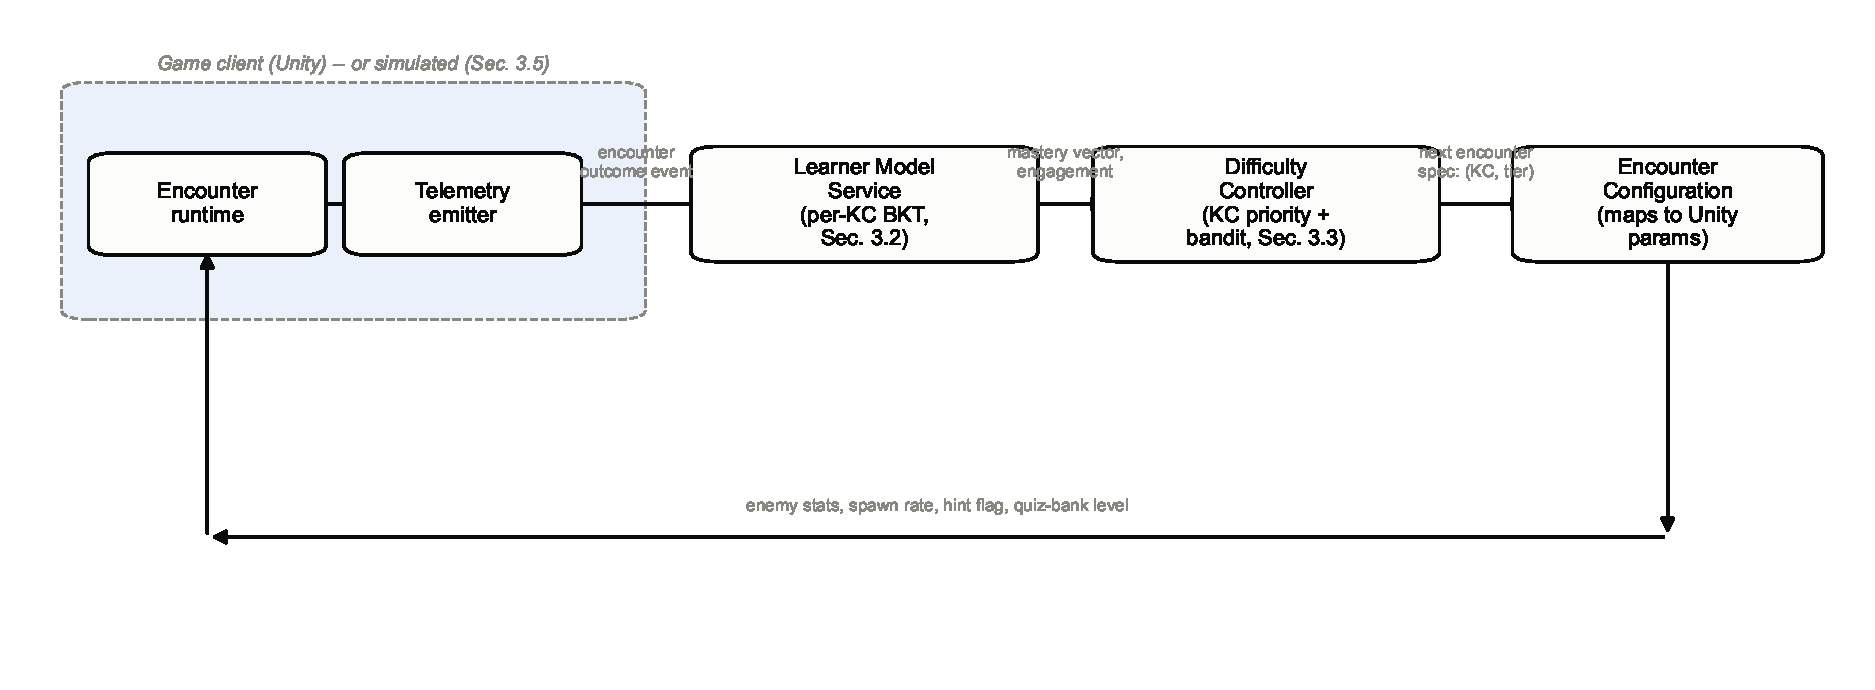
\includegraphics[width=\textwidth]{figures/figure4_architecture.pdf}
\caption{System architecture: the AI layer as a service outside the Unity client (or the offline simulation harness), communicating via one event schema.}
\label{fig:architecture}
\end{figure}

Event schema (per encounter): \texttt{\{learner\_id, timestamp, kc, difficulty\_tier, quiz\_outcome?, combat\_outcome, response\_latency\_ms, retries\}}. The \texttt{quiz\_outcome} field is optional because not every encounter includes a quiz/dialogue check; \texttt{combat\_outcome} is always present.

Only the Encounter Runtime / Telemetry Emitter box is Unity-specific; the Learner Model Service, Difficulty Controller, and Encounter Configuration are implemented as plain, engine-independent code (Section 3.5), which is what makes a pure-simulation evaluation possible before the full Unity integration exists.
%TODO: state explicitly here (and in Section 5.3) that the current Unity build (Level 1) does not yet emit this event schema.

\subsection{Simulation methodology}

\textbf{Synthetic learner agents.} Each simulated learner $i$ has, per KC $k$, a true latent skill $s_{i,k} \in [0,1]$ (distinct from the model's \textit{estimate} of it), a learning rate $\alpha_{i,k}$, and a forgetting rate $\varphi_{i,k}$, each drawn from distributions (e.g., skill $\sim$ Beta, rates $\sim$ truncated Normal) to represent a heterogeneous classroom population rather than a single archetype.

\textbf{Response generation.} Given an encounter at difficulty tier $d$ (mapped to a numeric difficulty value on the same $[0,1]$ scale as skill) for KC $k$, the probability of a successful outcome follows a two-parameter logistic item-response function \cite{ref27}:
\begin{equation}
P(\text{success}) = \sigma\big(\beta\,(s_{i,k} - d)\big)
\end{equation}
with slope $\beta$ controlling how sharply success probability changes around the skill--difficulty crossover, floored/ceilinged by small guess/slip constants so that success is never exactly 0 or 1. After each attempt, true skill updates stochastically toward mastery at rate $\alpha_{i,k}$ if the attempt was a genuine learning opportunity (not a pure guess/slip outcome), and decays at rate $\varphi_{i,k}$ per unit of elapsed time without practicing that KC.

\textbf{Engagement dynamics.} A simple accumulator tracks frustration (triggered by a run of low-success encounters) and boredom (triggered by a run of high-success encounters); both reduce the effective learning rate $\alpha_{i,k}$, giving the simulation a mechanism by which poor difficulty matching plausibly harms learning, not just enjoyment -- this is what makes the challenge--skill-balance metric below meaningful rather than cosmetic.

\textbf{Experimental design.} A population of $N{=}200$ synthetic learners is played through a fixed-length session of 120 encounters under four conditions (120 encounters raised from an initial plan of 60: at 60, true skill essentially never reached threshold within the session for any condition, a structural artifact of per-KC exposure rather than a tuning problem -- see Section 4):
\begin{enumerate}
\item \textbf{Static baseline} -- the original fixed level/stage/boss progression and fixed per-stage difficulty, i.e., no controller.
\item \textbf{Full adaptive} -- mastery-based KC selection + bandit tier selection (Sections 3.2--3.3).
\item \textbf{Ablation} -- mastery-based KC selection with \textit{random} tier selection, to isolate how much of the effect comes from targeting the right concept versus from tuning difficulty within it.
\item \textbf{Static, well-tuned} -- the same fixed rotation as condition 1, but every KC assigned the single population-appropriate tier rather than the original per-KC assignment (Section 4.8).
\end{enumerate}

\textbf{Metrics.}
\begin{itemize}
\item \textit{Time-to-mastery} per KC: encounters until the same sustained-crossing rule used by the controller ($m{=}10$ consecutive practiced encounters at or above $\theta{=}0.7$, Section 3.3) is satisfied, computed separately for the model estimate $P(L_k)$ and for true skill $s_k$, so the two can be compared under an identical definition of ``mastered'' and applied uniformly across all conditions, including the static baseline (which does not use this rule to make decisions, but is scored by it for a fair comparison).
\item \textit{Final mastery} across all five KCs at session end.
\item \textit{Challenge--skill balance}: proportion of encounters whose realized success rate fell inside the target flow band.
\item \textit{Engagement trajectory}: accumulated frustration/boredom over the session.
\item \textit{Estimator calibration}: correlation and calibration curve between the model's $P(L_{k,t})$ and the simulation's ground-truth $s_{i,k}$ -- a check that is only possible in simulation (ground truth is unobservable with real learners), and worth reporting precisely because it validates the knowledge-tracing model's core assumption before any real deployment.
\end{itemize}

Section 4 reports these metrics from the implemented simulation (Python, engine-independent per Section 3.4; code and full output available per the Data Availability Statement).

\section{Results}

All results below are from the simulation described in Section 3.5 ($N{=}200$ synthetic learners per replication, 120 encounters). Table~\ref{tab:table1} reports each condition-level metric as mean $\pm$ SD across 15 independent replications (different random seeds, each a fresh population of 200 synthetic learners), rather than a single run, so the spread reflects genuine run-to-run variability, not just within-population averaging.

\begin{table}[h]
\centering
\caption{Condition-level metrics, mean $\pm$ SD over 15 replications (200 learners each), with the confirmation-streak requirement $m{=}10$.}
\label{tab:table1}
\begin{tabular}{@{}lcccc@{}}
\toprule
Condition & Challenge--skill balance & Calibration ($r$) & Frustration & Boredom \\
\midrule
Static baseline & $0.219 \pm 0.005$ & $0.753 \pm 0.010$ & $0.208 \pm 0.006$ & $0.240 \pm 0.006$ \\
\textbf{Full adaptive} & $\mathbf{0.356 \pm 0.003}$ & $0.698 \pm 0.005$ & $\mathbf{0.124 \pm 0.010}$ & $0.040 \pm 0.002$ \\
Ablation (random tier) & $0.260 \pm 0.003$ & $0.672 \pm 0.007$ & $0.270 \pm 0.011$ & $0.029 \pm 0.002$ \\
\bottomrule
\end{tabular}
\end{table}

\begin{figure}[h]
\centering
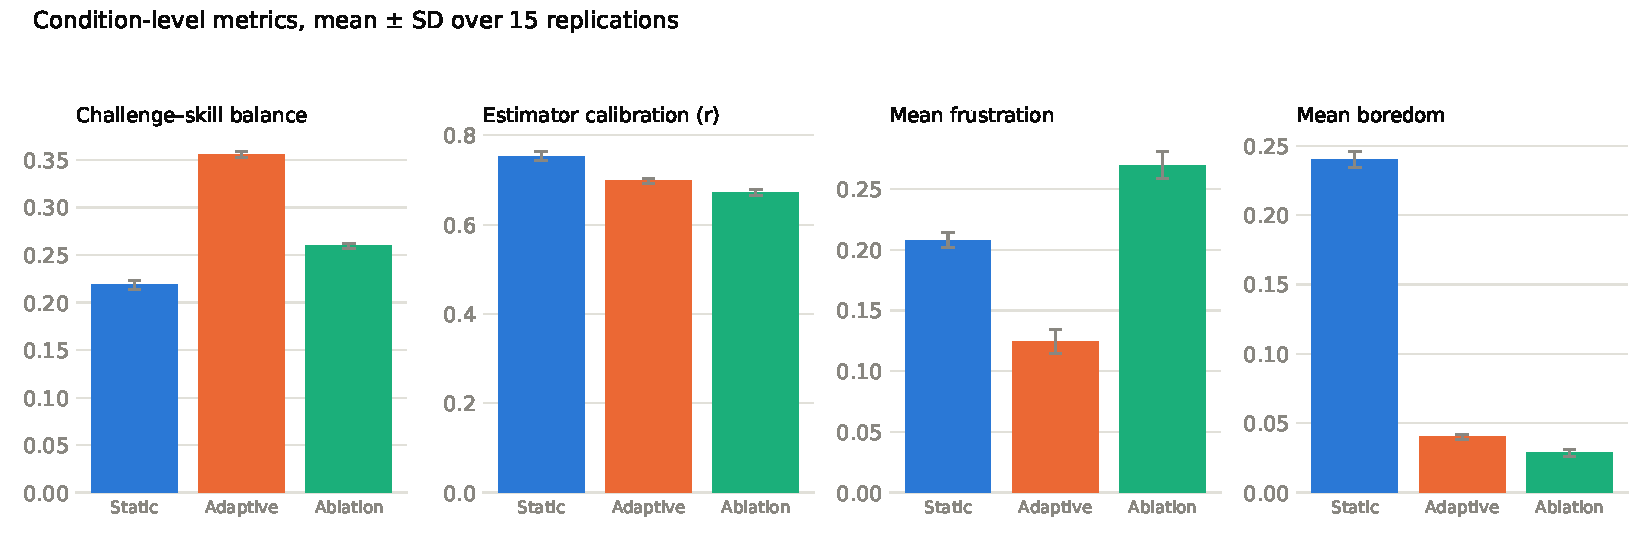
\includegraphics[width=0.85\textwidth]{figures/figure2_condition_metrics.pdf}
\caption{Condition-level metrics, mean $\pm$ SD over 15 replications, corresponding to Table~\ref{tab:table1}. Colors are consistent across every figure in this paper: blue = static baseline, orange = full adaptive, aqua = ablation (random tier).}
\label{fig:table1chart}
\end{figure}

Every condition pair is cleanly separated (non-overlapping min--max ranges across the 15 replications) on all four metrics at this setting. Two things are worth noting relative to an earlier pass of this analysis using a shorter confirmation requirement ($m{=}3$, since revised -- see Section 4.7): full adaptive's frustration advantage over static, previously modest and non-robust, is now clearly robust ($0.124 \pm 0.010$ vs.\ $0.208 \pm 0.006$, no overlap); and full adaptive's boredom, while still far below static's, has risen from $\approx 0.01$ to $0.040 \pm 0.002$ -- a real cost of requiring more sustained evidence before moving on from an already-learned concept, reported rather than omitted.

\subsection{Estimator calibration}

The knowledge tracing model's mastery estimate correlates with true simulated skill at $r{=}0.753$ under the static baseline and $r \approx 0.67$--$0.70$ under the two conditions that use the estimate to make decisions (full adaptive, ablation) -- closer than in an earlier pass of this analysis ($r \approx 0.58$--$0.60$ under a shorter, $m{=}3$ confirmation requirement; Section 4.7), consistent with our candidate explanation that the confirm-and-revoke practice pattern specific to mastery-based selection (Section 3.3) is a source of estimate/true-skill mismatch: a longer required streak reduces how often a KC is confirmed, revoked by forgetting, and re-practiced, producing a smoother relationship between logged estimate and true skill than the shorter requirement did. We have not formally isolated this mechanism beyond this one supporting observation, so it remains the most plausible candidate explanation rather than a demonstrated one. Either way, a correlation in the 0.67--0.75 range is positive and usable but not perfect, which is the basis for treating the hand-set BKT parameters (Section 3.2) as provisional rather than deployment-ready -- reinforced directly by Section 4.7's premature-mastery-declaration finding.

\subsection{Challenge--skill balance and engagement}

The full adaptive condition places 35.6\% of encounters inside the target flow band on average, compared with 26.0\% for the ablation and only 21.9\% for the static baseline (Table~\ref{tab:table1}) -- consistent with the intended effect of the bandit-based tier controller (Section 3.3), and robust across all 15 replications. Boredom shows the opposite failure mode, and both mastery-priority conditions avoid most of it (0.040 for full adaptive, 0.029 for ablation, versus 0.240 for static), because static's fixed rotation keeps re-serving already-strong KCs long after they stop being challenging; full adaptive's boredom is nonetheless several times higher than the near-zero level observed under a shorter confirmation requirement (Section 4.7), the direct cost of waiting out ten consecutive above-threshold observations on a concept that may already be effectively learned. Mean frustration is clearly and robustly lowest under full adaptive, including against the static baseline (0.124 vs.\ 0.208, no overlap across 15 replications) -- unlike in an earlier pass of this analysis, where the advantage over static specifically was modest and non-robust; the frustration advantage over the ablation remains large and robust (0.124 vs.\ 0.270).

\subsection{The difficulty trap in the static baseline}

\begin{table}[h]
\centering
\caption{Final mastery per knowledge component (mean across 200 learners). Model / true.}
\label{tab:table2}
\begin{tabular}{@{}lccc@{}}
\toprule
KC & Static & Full adaptive & Ablation \\
\midrule
Innate immunity & 1.00 / 0.68 & 0.97 / 0.75 & 0.94 / 0.71 \\
Antigen recognition & 1.00 / 0.68 & 0.97 / 0.74 & 0.93 / 0.70 \\
Cell-mediated immunity & 0.87 / 0.76 & 0.96 / 0.75 & 0.94 / 0.70 \\
Humoral immunity & 0.90 / 0.79 & 0.96 / 0.75 & 0.95 / 0.71 \\
Tolerance \& autoimmunity & 0.22 / 0.40 & 0.97 / 0.75 & 0.94 / 0.69 \\
\midrule
\textbf{Range (true skill)} & \textbf{0.39} & \textbf{0.01} & \textbf{0.02} \\
\bottomrule
\end{tabular}
\end{table}

\begin{figure}[h]
\centering
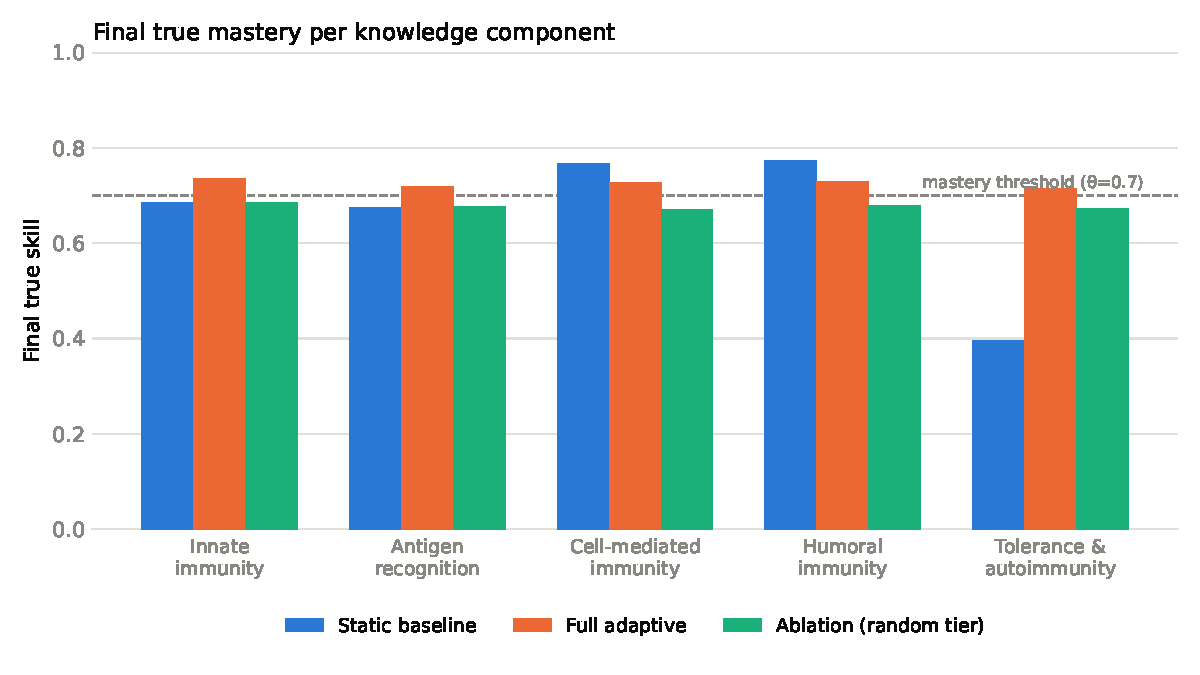
\includegraphics[width=0.85\textwidth]{figures/figure1_final_mastery.pdf}
\caption{Final true mastery per knowledge component, corresponding to Table~\ref{tab:table2}. The dashed line marks the mastery threshold $\theta{=}0.7$.}
\label{fig:table2chart}
\end{figure}

Under the static baseline -- the original game's fixed level order and fixed per-stage difficulty (Section 3.1) -- final true mastery ranges from 0.68--0.79 for four KCs to just 0.40 for tolerance/autoimmunity, the KC permanently assigned the ``Hard'' tier as the final-boss encounter. The model's own estimate for that KC (0.22) is, unusually, an \textit{under}-estimate relative to true skill (0.40) rather than the over-estimation seen elsewhere in this paper. It is well above the 0.1 prior (Section 3.2) -- the unconditional per-attempt learning-transit term still pulls it upward regardless of correctness -- but far below both true skill and the 0.87--1.00 estimates reported for the other four KCs under static, consistent with an encounter difficulty so mismatched to typical learner skill that observations are predominantly ``incorrect'' and rarely informative, leaving the two competing pulls (transit upward, evidence downward) roughly balanced at a low value rather than resolving toward either extreme. This is the ``difficulty trap'' referenced in the Introduction: a fixed difficulty assignment that happens to be badly matched to a KC leaves that KC under-served regardless of how many attempts a learner makes at it, because the encounters generated are rarely informative learning opportunities for a learner starting well below that difficulty (Section 3.5).

\begin{figure}[h]
\centering
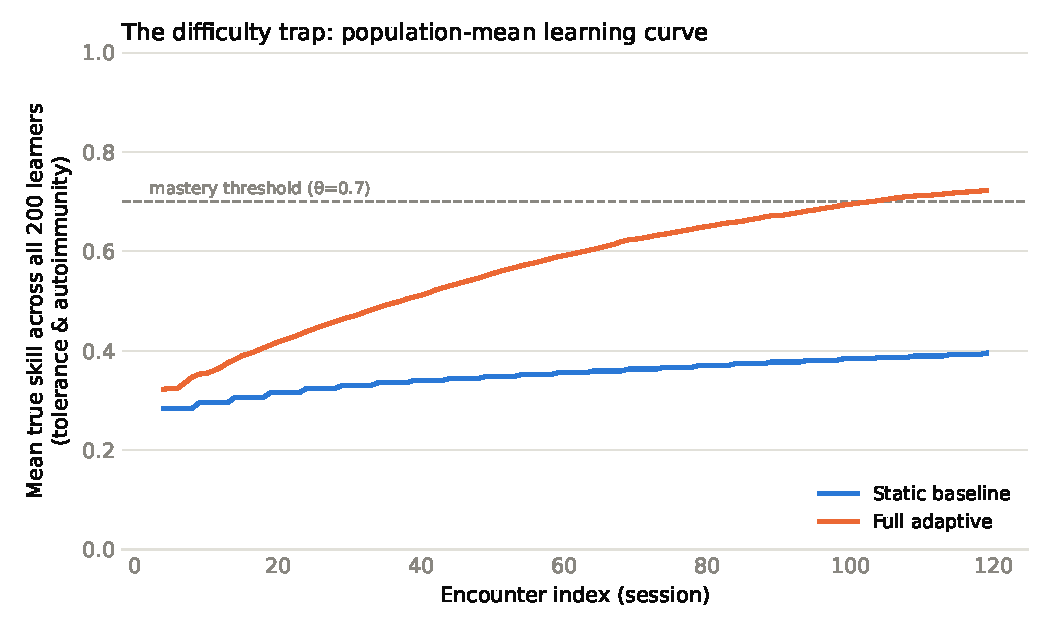
\includegraphics[width=0.85\textwidth]{figures/figure3_difficulty_trap_trajectory.pdf}
\caption{Mean true skill on tolerance \& autoimmunity across all 200 learners over the course of the session, static baseline vs.\ full adaptive. Static plateaus well below threshold; full adaptive crosses it around encounter 100.}
\label{fig:trajectory}
\end{figure}

\subsection{Equity across concepts under mastery-based sequencing}

Both conditions that use mastery-based KC selection (full adaptive and the ablation) reduce the true-skill range across the five KCs to 0.01--0.02 in the representative run (Table~\ref{tab:table2}). Across all 15 replications this is one of the paper's most robust findings (see also Section 4.8): mean range $0.373 \pm 0.028$ under static versus $0.016 \pm 0.006$ (full adaptive) and $0.015 \pm 0.004$ (ablation) -- roughly a 23- to 25-fold reduction in cross-concept inequality, with no overlap between static and either mastery-based condition across any of the 15 runs. Full adaptive and the ablation are statistically indistinguishable from each other on this specific metric (overlapping ranges), confirming that the equity gain is a property of mastery-based KC selection itself, not of the difficulty-tier bandit -- no KC is left behind under either mastery-priority condition.

With the confirmation-streak requirement at its current value ($m{=}10$, Section 4.7), this equity gain is not achieved at a meaningful cost to peak performance: full adaptive reaches 0.74--0.75 true skill on every KC (Table~\ref{tab:table2}), matching or nearly matching static's two best-served concepts (0.76, 0.79) while dramatically correcting its worst (0.40 $\to$ 0.75), and exceeding static's two moderately-served concepts (0.68, 0.68) outright. The one residual gap is small -- static's single best concept (humoral immunity, 0.79) still edges out full adaptive's uniform 0.75 by 0.04 -- but this is a minor asymmetry, not the substantial equity/peak-performance trade-off reported in an earlier pass of this analysis under a shorter confirmation requirement. That earlier trade-off turned out to be largely an artifact of $m{=}3$ confirming (and thus abandoning further practice on) concepts too early, rather than an inherent property of mastery-based sequencing; Section 4.7 discusses this directly.

\subsection{Isolating the bandit's contribution}

Per-KC time-to-sustained-mastery is reported in full in Supplementary Table S1 rather than in the main text: with $m{=}10$ required consecutive above-threshold observations, this metric is heavily censored under every condition (27--94\% of learners never accumulate a full confirmation streak within the 120-encounter session, even on concepts where Table~\ref{tab:table2} shows they have in fact reached a high true skill level), which makes the exact ``mean encounters among those who confirmed'' figures a weaker, selection-biased basis for comparison than Table~\ref{tab:table2}'s final-mastery levels. The one robust, aggregate pattern is kept here because it is not subject to the same selection-bias concern -- the \textit{censoring rate itself}: static's censoring ranges from 1\% to 94\% depending on how well-matched that concept's fixed difficulty happens to be, while full adaptive is consistently in a narrow 27--30\% band across all five concepts, and the ablation is consistently worse still (64--67\%).

The ablation shares full adaptive's mastery-based KC-selection rule but replaces the bandit with a uniformly random tier choice. It no longer quite matches full adaptive's final true skill (0.69--0.71 vs.\ 0.74--0.75, Table~\ref{tab:table2}) or its equity outcome as tightly (range 0.02 vs.\ 0.01), and is both slower to confirm (64--67\% censored vs.\ 27--30\%) and, per Section 4.2, more frustrating throughout (0.270 vs.\ 0.124). Combined with the challenge--skill-balance and frustration results, this isolates concept sequencing as the primary source of the equity gain, and difficulty-tier adaptation as the source of the additional efficiency, engagement, and final-mastery-level gains full adaptive achieves over the ablation.

\subsection{Robustness beyond the reported parameter setting}

Two further checks address a specific concern with any simulation-only evaluation: that the same assumptions used to build the system were also used to build the world it is tested in, and that the reported parameters may have been implicitly selected because they produced a favorable result.

\textbf{Cross-model check.} The 15-replication comparison uses synthetic learners whose true success probability follows a clean logistic curve -- the same functional family the difficulty tiers were designed around. To test whether the result depends on this match, we re-ran all three conditions (5 seeds, 200 learners each) with an added per-attempt perturbation representing ``good/bad day'' variability, unrelated to any assumption in the knowledge tracing model or the bandit's reward shaping. The equity finding was essentially unchanged (mean cross-concept inequality: static 0.231, full adaptive 0.015, ablation 0.019), indicating it is not an artifact of the AI being well-matched to its own test world. The challenge--skill-balance ranking was less stable under this perturbation: full adaptive remained best (0.326), but the ablation dropped below static (0.257 vs.\ 0.287) rather than sitting between static and full adaptive as in the clean-world result -- reported here rather than omitted.

\textbf{Sensitivity sweep.} Varying the response-curve steepness (IRT slope 4/6/8) and the knowledge-tracing learning-transit rate (0.04/0.06/0.10) one at a time, single seed per setting, left the equity finding intact at every setting tested: static's cross-concept inequality exceeded both mastery-based conditions by at least a factor of 10 in every one of the five distinct settings tested, with no exceptions. The challenge--skill-balance ranking (full adaptive $>$ ablation $>$ static) also held at every setting tested. Full detail and code: \texttt{simulation/robustness\_checks.py}.

\subsection{How much does the confirmation-streak rule actually help?}

We quantified directly, rather than leaving it as a qualitative development anecdote, how often the controller declares a KC mastered while true skill is still below threshold, across every KC-confirmation event logged under full adaptive (5 seeds, 200 learners each) (Table~\ref{tab:table3}).

\begin{table}[h]
\centering
\caption{Premature-declaration rate by confirmation-streak length $m$.}
\label{tab:table3}
\begin{tabular}{@{}lcc@{}}
\toprule
$m$ & Premature-declaration rate & KC-confirmations observed \\
\midrule
1 (single crossing) & 92.8\% & 4999 \\
3 (an earlier pass of this analysis) & 72.3\% & 4929 \\
\textbf{10 (used throughout this paper)} & \textbf{15.4\%} & 3370 \\
\bottomrule
\end{tabular}
\end{table}

We did not stop at the first improvement ($m{=}3$): a broader sweep ($m{=}1,3,5,7,10,15,20$) showed premature declarations continuing to fall well past $m{=}3$, alongside a separate check that raising $m$ further did not damage the other headline metrics -- estimator calibration and frustration in fact \textit{improved} and the equity finding was essentially unaffected -- at the cost of a real but modest rise in boredom and heavier censoring of the time-to-mastery metric specifically. $m{=}10$ was selected as the point past which returns diminish sharply (the sample of observed confirmations available to even measure this rate shrinks quickly beyond $m{=}10$, e.g., to 1303 at $m{=}15$) rather than as a value chosen to make a favorable result look better.

Even at $m{=}10$, the confirmation-streak requirement reduces premature mastery declaration substantially (92.8\% $\to$ 15.4\%, an 83\% relative reduction) but does not eliminate it: roughly one in six concepts the system reports as ``confirmed mastered'' is not, by the simulation's own ground truth, actually mastered yet. Full detail and code: \texttt{simulation/premature\_mastery\_check.py}.

\subsection{How much of the static baseline's disadvantage is an avoidable design choice?}

The static baseline mirrors the original game's own difficulty assignment, which happens to place a mismatched ``Hard'' tier on one concept. Because every knowledge component in this simulation draws initial skill from the same distribution, there is no population-level reason a fixed baseline should treat any concept differently -- the original mismatch is an arbitrary property of the game's design, not a necessary feature of non-adaptive difficulty. To separate these, we tested a \textbf{well-tuned static baseline}: the same fixed rotation, but every concept assigned the single uniform tier that best serves this population (Easy, Medium, and Hard were each tested across 15 replications; Medium dominated on every metric).

\begin{table}[h]
\centering
\caption{Well-tuned static baseline (uniform Medium tier) vs.\ the other three conditions, mean $\pm$ SD over 15 replications.}
\label{tab:table4}
\begin{tabular}{@{}lcccccc@{}}
\toprule
Condition & CSB & Calib.\ ($r$) & Frustration & Boredom & Mastery range & Mean final true skill \\
\midrule
Static (mismatched) & 0.219 $\pm$ 0.005 & 0.753 $\pm$ 0.010 & 0.208 $\pm$ 0.006 & 0.240 $\pm$ 0.006 & 0.373 $\pm$ 0.028 & 0.662 \\
\textbf{Static, well-tuned} & 0.337 $\pm$ 0.007 & \textbf{0.844 $\pm$ 0.004} & 0.186 $\pm$ 0.004 & 0.141 $\pm$ 0.005 & 0.032 $\pm$ 0.008 & \textbf{0.765 $\pm$ 0.004} \\
Full adaptive & 0.356 $\pm$ 0.003 & 0.698 $\pm$ 0.005 & \textbf{0.124 $\pm$ 0.010} & 0.040 $\pm$ 0.002 & \textbf{0.016 $\pm$ 0.006} & $\approx$0.748 \\
Ablation & 0.260 $\pm$ 0.003 & 0.672 $\pm$ 0.007 & 0.270 $\pm$ 0.011 & 0.029 $\pm$ 0.002 & 0.015 $\pm$ 0.004 & $\approx$0.702 \\
\bottomrule
\end{tabular}
\end{table}

Picking a single sensible fixed difficulty closes most of the equity gap on its own -- an 11.6-fold reduction in cross-concept inequality (0.373 $\to$ 0.032) from a change that adapts nothing at runtime, confirming that a substantial share of the original static baseline's disadvantage (Section 4.4) was avoidable rather than inherent to non-adaptive difficulty. The well-tuned baseline also reaches the \textit{highest} mean final mastery and calibration of any of the four conditions tested, including full adaptive. Full adaptive's genuine remaining advantages over a well-designed non-adaptive alternative are narrower and more specific than the comparison against the original (mismatched) static baseline alone would suggest: full adaptive still wins clearly on frustration (0.124 vs.\ 0.186) and on the residual equity gap (0.016 vs.\ 0.032, roughly half), but it does not win on raw final mastery level or on estimator calibration. We read this as full adaptive's advantage coming specifically from \textbf{personalizing to the individual learner} rather than merely improving on a population-level policy -- a well-tuned fixed difficulty already captures most of what population-level tuning can offer, and the remaining gap is what adapting to each learner's own trajectory adds on top. It is also worth noting plainly that identifying ``Medium'' as the right uniform tier required exactly the kind of systematic sweep a real deployment would not have access to in advance; an adaptive system's practical advantage includes not needing that sweep at all. Full detail and code: \texttt{simulation/well\_tuned\_baseline\_check.py}.

\section{Discussion}

\subsection{Interpretation relative to prior work}

The central finding -- that a fixed difficulty assignment can leave one concept severely under-mastered regardless of attempt count, while mastery-based sequencing corrects this -- is consistent with, and gives a concrete instance of, the general critique of static content authoring in the games-adaptivity literature \cite{ref3,ref24} and with the motivation behind knowledge tracing in intelligent tutoring systems more broadly \cite{ref16,ref17}. What this paper adds beyond restating that critique is a specific mechanism decomposition: the ablation (Section 4.5) shows the equity gain and the efficiency/engagement gain are separable and attributable to different components (mastery-based concept selection versus difficulty-tier adaptation, respectively). This distinction matters for design: a system builder constrained to implement only one adaptive mechanism should, on this evidence, prioritize concept-level sequencing for equity, but should not expect that alone to deliver the efficiency and frustration benefits typically attributed to ``adaptive difficulty'' in the DDA literature \cite{ref22,ref23} -- those specifically required the bandit-based tier controller. The equity framing itself connects to a strand of the knowledge-tracing literature concerned with fairness across learners for a given skill \cite{ref34,ref35} (Section 2.2); this paper's equity finding is the same concern rotated ninety degrees -- fairness \textit{across concepts} for a given learner, rather than across learners for a given concept.

The estimator-calibration correlations ($r \approx 0.67$--$0.75$) are in line with the general caution in the knowledge-tracing literature that simpler models such as BKT trade some accuracy for interpretability and data efficiency \cite{ref19}, and reinforce a point made in Section 3.3's design rationale: a sequencing policy that trusts a single above-threshold observation from an imperfectly calibrated estimator can withdraw instruction prematurely. Section 4.7 quantifies this directly: a single-crossing rule declares a concept mastered while true skill is still below threshold 92.8\% of the time; requiring ten consecutive above-threshold observations reduces this to 15.4\% -- substantial, and the setting used throughout this paper's other results, but not a solved problem.

\subsection{Revisiting the equity--peak-performance question}

An earlier pass of this analysis, using a shorter confirmation-streak requirement ($m{=}3$), found mastery-based sequencing reduced cross-concept inequality substantially but at a real cost to peak performance: full adaptive reached only 0.61--0.63 true skill on every concept, well below static's best-served concepts (0.76--0.79). Raising the confirmation requirement to $m{=}10$ -- motivated independently, by the premature-declaration problem in Section 4.7, not by this trade-off -- mostly dissolved it. In hindsight, the original trade-off was largely an artifact of $m{=}3$ causing the controller to confirm -- and therefore stop practicing -- concepts too early, not an inherent property of mastery-based sequencing itself. Section 4.8 complicates this picture further and, we think, productively: once static is given its best possible fixed policy rather than the original mismatched one, it matches or exceeds full adaptive on peak performance \textit{and} on equity is only a factor of two behind, not an order of magnitude. The honest updated version of this section's question is not ``does equity cost peak performance'' but ``what, specifically, does personalization buy beyond a well-tuned population-level policy'' -- and Section 4.8's answer (lower frustration, a smaller residual equity gap, and not needing to already know the right fixed policy) is narrower than what an earlier pass of this paper would have claimed.

\subsection{Limitations}

\begin{itemize}
\item \textbf{Simulation-only evaluation.} Every quantitative result in Section 4 is generated from synthetic learner agents whose behavior follows a model we specified, not from real learners. No amount of further simulation changes this; only real pilot or classroom data can.
\item \textbf{Same-author risk in system and evaluation design.} The AI system and the synthetic world used to test it were designed by the same authors. Section 4.6's cross-model check is a partial mitigation but does not eliminate the concern.
\item \textbf{Hand-set rather than data-fit parameters.} The knowledge tracing and synthetic-learner parameters were set to plausible values, not fit to any real dataset. The sensitivity sweep shows the qualitative equity finding is not fragile to the exact values chosen, but this is not a substitute for calibration against real play data.
\item \textbf{A well-tuned static baseline narrows, but does not close, full adaptive's advantage -- and changes what that advantage actually consists of.} Section 4.8's finding is a real refinement of this paper's central claim, not only a limitation.
\item \textbf{The game client does not yet implement the architecture described in Section 3.4.} Only Level 1 of the Unity build exists at the time of writing, and it does not emit the telemetry event schema the AI layer depends on.
\item \textbf{Premature mastery declaration is reduced, not solved.} Roughly one in six confirmations are still premature even under the improved $m{=}10$ rule.
\item \textbf{The time-to-mastery metric is heavily censored at $m{=}10$.} Table~S1's per-KC breakdown should be read as secondary to Table~\ref{tab:table2}.
\item \textbf{A narrow design space was tested.} Five knowledge components, three difficulty tiers, and one specific controller design were evaluated; we do not claim this is the best possible design.
\end{itemize}

\subsection{Future work}

The limitations above point directly to next steps: (1) complete the Unity client's telemetry emitter and wire it to the architecture in Section 3.4; (2) extend the well-tuned-baseline analysis (Section 4.8) to a per-learner-matched fixed policy to test whether personalization specifically, rather than adaptivity generally, is what closes the residual gap identified there; (3) collect a small amount of real play or quiz-response data to fit the knowledge tracing parameters currently set by hand, which would also let $m$ be validated or re-tuned against real evidence; (4) test a longer session length to establish whether the Table~S1 censoring problem reflects a genuinely slow confirmation process or simply an under-sized session budget; and (5) run a small classroom pilot with real learners aged 8--16, requiring age-appropriate consent/assent procedures and institutional ethics review. Beyond validation, the architecture in Section 3.4 is not specific to immunology or to this game's mechanics, and extending the concept-to-encounter mapping to other biology or STEM topics, or replacing the fixed quiz bank with generative-AI-produced content and feedback \cite{ref1,ref2,ref10}, are natural directions consistent with the broader aims of this special issue.

\section{Conclusions}

This paper presented the design, implementation, and simulation-based evaluation of an AI layer for immune-system serious games, coupling a two-channel Bayesian knowledge tracing model with a mastery-priority, bandit-driven adaptive difficulty controller, built on top of the existing (partially implemented) \textit{Immune Soldiers} game \cite{ref9}. Rather than assuming an adaptive layer would simply outperform the original fixed-difficulty design, we tested that assumption through an escalating series of checks -- an ablation isolating the difficulty-tier bandit's specific contribution, a 15-replication robustness analysis, a cross-model check, a parameter sensitivity sweep, and a well-tuned-baseline comparison -- each designed to surface where the system's benefits do and do not hold, rather than to confirm a single favorable result.

The central finding is that the original game's fixed difficulty assignment creates a genuine ``difficulty trap'': a concept assigned a poorly matched difficulty tier is left severely under-mastered no matter how many attempts a learner makes, while mastery-based concept sequencing corrects this specific failure. This correction was only achieved without a meaningful cost to already-well-served concepts after we identified and addressed a more fundamental problem: an imperfectly calibrated knowledge-tracing estimator can cause an adaptive system to withdraw instruction before a concept is genuinely learned. Requiring ten consecutive above-threshold observations rather than one reduced this from 92.8\% to 15.4\% of confirmations being premature -- a substantial improvement, but not a complete fix. A further test showed that much of the original baseline's disadvantage was an avoidable design choice rather than an inherent property of non-adaptive difficulty; the adaptive system's genuine remaining advantage is narrower and more specific -- lower frustration and a smaller residual equity gap from personalizing to each learner -- than a comparison against only the original baseline would have suggested.

We report this as what it is: a first, simulation-validated technical contribution, not a demonstration of real educational efficacy. Every quantitative result in this paper describes how the system behaves against synthetic learners whose behavior we specified; its value for real students aged 8--16 remains untested. What we believe this paper does establish is that knowledge tracing and adaptive difficulty can be combined for a specific serious-game domain in a way that is auditable, whose individual mechanisms can be isolated and independently justified, and whose limitations are quantified rather than assumed away -- a more modest contribution than a headline claim of improved learning, but, we think, a more trustworthy one.

\section*{Supplementary Materials}
Table S1: Time-to-sustained-mastery in encounters per knowledge component (model estimate; mean across learners reaching it; \% never reaching it within the 120-encounter session in parentheses).

\begin{table}[h]
\centering
\begin{tabular}{@{}lccc@{}}
\toprule
KC & Static & Full adaptive & Ablation \\
\midrule
Innate immunity & 59.3 (1\%) & 93.7 (28\%) & 95.5 (66\%) \\
Antigen recognition & 62.0 (2\%) & 93.0 (30\%) & 95.5 (66\%) \\
Cell-mediated immunity & 84.2 (36\%) & 93.9 (28\%) & 94.6 (64\%) \\
Humoral immunity & 83.4 (31\%) & 93.0 (30\%) & 93.7 (67\%) \\
Tolerance \& autoimmunity & 99.5 (94\%) & 95.2 (27\%) & 95.5 (64\%) \\
\bottomrule
\end{tabular}
\end{table}

\section*{Author Contributions}
Conceptualization, H.M.H.\ and A.T.; Methodology, H.M.H.; Software, H.M.H.; Validation, H.M.H.\ and O.T.; Formal Analysis, H.M.H.; Investigation, H.M.H.\ and O.T.; Resources, O.T.; Data Curation, H.M.H.; Writing -- Original Draft Preparation, H.M.H.; Writing -- Review \& Editing, H.M.H., O.T.\ and A.T.; Visualization, H.M.H.; Supervision, A.T.; Project Administration, A.T.
%TODO: this is a plausible-default guess, not verified -- confirm actual role split, especially for O.T.

\section*{Funding}
[This research received no external funding. --- CONFIRM] %TODO

\section*{Data Availability Statement}
The simulation code, raw output, and figure-generation scripts supporting the findings of this study are openly available on GitHub at \url{https://github.com/HananHelwa/immune-soldiers-adaptive-difficulty}.
%TODO: consider archiving via Zenodo's GitHub integration for a citable DOI before final submission.

\section*{Acknowledgments}
The authors thank the original \textit{Immune Soldiers} development team --- Khalil Khalil (Munir) Dar Omar, Rami Said Khader, and Omar Adwan --- and their graduation-project supervisor, Dr. Radwan Kasrawi, for the design and development of the base game \cite{ref9} on which this paper's AI layer was built.

\section*{Conflicts of Interest}
The authors declare no conflicts of interest.

\begin{thebibliography}{99}

\bibitem{ref1} Li, H.; Xu, T.; Zhang, C.; Chen, E.; Liang, J.; Fan, X.; Li, H.; Tang, J.; Wen, Q. Bringing Generative AI to Adaptive Learning in Education. arXiv:2402.14601, 2024.
\bibitem{ref2} Wang, S.; Xu, T.; Li, H.; Zhang, C.; Liang, J.; Tang, J.; Yu, P.S.; Wen, Q. Large Language Models for Education: A Survey and Outlook. arXiv:2403.18105, 2024.
\bibitem{ref3} Tripathi, P.; Kapralos, B. AI-Enabled Serious Games: Integrating Intelligence and Adaptivity in Training Systems. arXiv:2605.21962, 2026.
\bibitem{ref4} Frutos-Pascual, M.; Garcia-Zapirain, B. Review of the Use of AI Techniques in Serious Games: Decision Making and Machine Learning. \textit{IEEE Transactions on Computational Intelligence and AI in Games} \textbf{2017}, \textit{9}, 133--152.
\bibitem{ref5} Stranford, S.A.; Owen, J.A.; Mercer, F.; Pollock, R.R. Active Learning and Technology Approaches for Teaching Immunology to Undergraduate Students. \textit{Frontiers in Public Health} \textbf{2020}, \textit{8}, 114.
\bibitem{ref6} Liberman, A.; Kario, D.; Mussel, M.; Brill, J.; Buetow, K.; Efroni, S.; Nevo, U. Cell studio: A platform for interactive, 3D graphical simulation of immunological processes. \textit{APL Bioengineering} \textbf{2018}, \textit{2}, 026107.
\bibitem{ref7} Konstantara, K.; Xinogalos, S. Cells of War: A Serious Game for Familiarizing Players With the Immune System. \textit{Simulation \& Gaming} \textbf{2018}, \textit{49}, 567--589.
\bibitem{ref8} Immune Attack [Video game]. Federation of American Scientists Learning Technologies Program, 2008. Available online: \url{https://web.archive.org/web/20161024120755/http://www.fas.org/immuneattack/} (accessed on 24 October 2016, archived snapshot).
\bibitem{ref9} Immune Soldiers Game Design Document, unpublished graduation project, Team ``Meet To Eat'' (H.M. Helwa, K.K. Dar Omar, R.S. Khader, O. Adwan); Al-Quds University, Ramallah, Palestine, supervised by Dr. Radwan Kasrawi. %TODO: confirm institution
\bibitem{ref10} Wermann, C.; Avila, K.E.; Andr\'e, S.; Draeger, J.C.; Goetze, A.; Kuhn, J.; Maurer, M.; Mehlhase, S.; Merkas, N.; Schrodt, F.; K\"uchemann, S. AI-based Verbal and Visual Scaffolding in a Serious Game: Effects on Learning and Cognitive Load. arXiv:2602.08893, 2026.
\bibitem{ref11} Arnab, S.; Lim, T.; Carvalho, M.B.; Bellotti, F.; de Freitas, S.; Louchart, S.; Suttie, N.; Berta, R.; De Gloria, A. Mapping learning and game mechanics for serious games analysis. \textit{British Journal of Educational Technology} \textbf{2015}, \textit{46}, 391--411.
\bibitem{ref12} Lameras, P.; Arnab, S.; Dunwell, I.; Stewart, C.; Clarke, S.; Petridis, P. Essential features of serious games design in higher education: Linking learning attributes to game mechanics. \textit{British Journal of Educational Technology} \textbf{2017}, \textit{48}, 972--994.
\bibitem{ref13} Abt, C. \textit{Serious Games}; Viking Press: New York, NY, USA, 1970.
\bibitem{ref14} Sawyer, B.; Rejeski, D. \textit{Serious Games: Improving Public Policy through Game-Based Learning and Simulation}; Woodrow Wilson International Center for Scholars: Washington, DC, USA, 2002.
\bibitem{ref15} Michael, D.; Chen, S. \textit{Serious Games: Games That Educate, Train, and Inform}; Course Technology: Boston, MA, USA, 2006.
\bibitem{ref16} Corbett, A.T.; Anderson, J.R. Knowledge tracing: Modeling the acquisition of procedural knowledge. \textit{User Modeling and User-Adapted Interaction} \textbf{1994}, \textit{4}, 253--278.
\bibitem{ref17} VanLehn, K. The relative effectiveness of human tutoring, intelligent tutoring systems, and other tutoring systems. \textit{Educational Psychologist} \textbf{2011}, \textit{46}, 197--221.
\bibitem{ref18} Piech, C.; Bassen, J.; Huang, J.; Ganguli, S.; Sahami, M.; Guibas, L.; Sohl-Dickstein, J. Deep knowledge tracing. In \textit{Advances in Neural Information Processing Systems 28 (NeurIPS 2015)}, 2015.
\bibitem{ref19} Shen, S.; Liu, Q.; Huang, Z.; Zheng, Y.; Yin, M.; Wang, M.; Chen, E. A Survey of Knowledge Tracing: Models, Variants, and Applications. \textit{IEEE Transactions on Learning Technologies} \textbf{2024}, \textit{17}, 1858--1882.
\bibitem{ref20} D'Mello, S.; Graesser, A. Dynamics of affective states during complex learning. \textit{Learning and Instruction} \textbf{2012}, \textit{22}, 145--157.
\bibitem{ref21} Baker, R.S.; Corbett, A.T.; Koedinger, K.R.; Wagner, A.Z. Off-task behavior in the cognitive tutor classroom: When students ``game the system.'' In \textit{Proceedings of the SIGCHI Conference on Human Factors in Computing Systems (CHI 2004)}, Vienna, Austria, 24--29 April 2004; pp. 383--390.
\bibitem{ref22} Hunicke, R. The case for dynamic difficulty adjustment in games. In \textit{Proceedings of the 2005 ACM SIGCHI International Conference on Advances in Computer Entertainment Technology (ACE 2005)}, Valencia, Spain, 15--17 June 2005.
\bibitem{ref23} Zohaib, M. Dynamic Difficulty Adjustment (DDA) in Computer Games: A Review. \textit{Advances in Human-Computer Interaction} \textbf{2018}, 2018, 5681652.
\bibitem{ref24} Lopes, R.; Bidarra, R. Adaptivity challenges in games and simulations: A survey. \textit{IEEE Transactions on Computational Intelligence and AI in Games} \textbf{2011}, \textit{3}, 85--99.
\bibitem{ref25} Sutton, R.S.; Barto, A.G. \textit{Reinforcement Learning: An Introduction}, 2nd ed.; MIT Press: Cambridge, MA, USA, 2018.
\bibitem{ref26} Csikszentmihalyi, M. \textit{Flow: The Psychology of Optimal Experience}; Harper \& Row: New York, NY, USA, 1990.
\bibitem{ref27} Embretson, S.E.; Reise, S.P. \textit{Item Response Theory for Psychologists}; Lawrence Erlbaum Associates: Mahwah, NJ, USA, 2000.
\bibitem{ref28} Stegman, M. Immune Attack players perform better on a test of cellular immunology and self-confidence than their classmates who play a control video game. \textit{Faraday Discussions} \textbf{2014}, \textit{169}, 403--423.
\bibitem{ref29} Lee, L.C.; Arakawa, Y.; Mine, T. Emerging Trends in Knowledge Tracing Models: A Technical Survey from 2022 to 2025. In \textit{Advanced Data Mining and Applications (ADMA 2025)}, Lecture Notes in Computer Science, vol. 16199; Springer: Singapore, 2025.
\bibitem{ref30} Rahimi, M.; Moradi, H.; Vahabie, A.; Kebriaei, H. Continuous Reinforcement Learning-based Dynamic Difficulty Adjustment in a Visual Working Memory Game. arXiv:2308.12726, 2023.
\bibitem{ref31} Tene, T.; Vique L\'opez, D.F.; Valverde Aguirre, P.E.; Cabezas Oviedo, N.I.; Vacacela Gomez, C.; Bellucci, S. A systematic review of serious games as tools for STEM education. \textit{Frontiers in Education} \textbf{2025}, \textit{10}, 1432982.
\bibitem{ref32} Badrinath, A.; Wang, F.; Pardos, Z.A. pyBKT: An Accessible Python Library of Bayesian Knowledge Tracing Models. In \textit{Proceedings of the 14th International Conference on Educational Data Mining (EDM 2021)}, 2021.
\bibitem{ref33} Nedungadi, P.; Remya, M.S. Incorporating forgetting in the Personalized, Clustered, Bayesian Knowledge Tracing (PC-BKT) model. In \textit{Proceedings of the 2015 International Conference on Cognitive Computing and Information Processing (CCIP)}, Noida, India, 2015; pp. 1--5.
\bibitem{ref34} Tschiatschek, S.; Knobelsdorf, M.; Singla, A. Equity and Fairness of Bayesian Knowledge Tracing. arXiv:2205.02333, 2022.
\bibitem{ref35} Stinar, F.; Lee, H.; Belitz, C.; Nasiar, N.; Fancsali, S.; Ritter, S.; Almoubayyed, H.; Baker, R.; Ocumpaugh, J.; Bosch, N. Fairness of Bayesian Knowledge Tracing for Math Learners of Different Reading Ability. In \textit{Proceedings of the 18th International Conference on Educational Data Mining (EDM 2025)}, Palermo, Italy, 2025.
\bibitem{ref36} Tao, X.; S\'aenz Lech\'on, N.; Eckert, M. Mapping the landscape of Artificial Intelligence for serious games in Health: An enhanced meta review. \textit{Computers in Human Behavior Reports} \textbf{2025}, \textit{18}, 100696.
\bibitem{ref37} Pistono, A.M.A.d.A.; dos Santos, A.M.P.; Baptista, R.J.V.; Mamede, H.S. Framework for adaptive serious games. \textit{Computer Applications in Engineering Education} \textbf{2024}, e22731.
\bibitem{ref38} Bloom, B.S. Learning for mastery. \textit{Evaluation Comment (UCLA Center for the Study of Evaluation of Instructional Programs)} \textbf{1968}, \textit{1}, 1--12.

\end{thebibliography}

\end{document}
